\documentclass{amsart}

\setlength{\textwidth}{13cm}
\setlength{\textheight}{19cm}

\usepackage{graphicx} 		% balik pro vkladani obrazku
\usepackage{amsmath, amsthm, amssymb}
%\usepackage{natbib}

%\usepackage[cp1250]{inputenc} 	% kodovani cestiny MS Windows
%\usepackage[latin2]{inputenc} 	% kodovani cestiny Linux
\usepackage[utf8]{inputenc}
\usepackage{comment}
\usepackage{xcolor}
  \usepackage{hyperref} % klikatelne odkazy v textu
  \hypersetup{
      colorlinks   = true, %Colours links instead of ugly boxes
      urlcolor     = blue, %Colour for external hyperlinks
      linkcolor    = red, %Colour of internal links
      citecolor   = red, %Colour of citations
      unicode=true % zajistí správné fungování háčků a čárek (češtiny) v PDF obsahu
    }

\newtheorem{theorem}{Theorem}
\newtheorem{corollary}[theorem]{Corollary}
\theoremstyle{definition}\newtheorem{definition}[theorem]{Definition}
\theoremstyle{remark}\newtheorem{remark}[theorem]{Remark}

\newcommand{\dif}{\,\mathrm{d}}
\newcommand{\e}{\,\mathrm{e}}
\newcommand{\E}{\,\mathrm{E}}
\newcommand{\D}{\,\mathrm{D}}
\newcommand{\ds}{\,\mathrm{d}s}
\newcommand{\dt}{\,\mathrm{d}t}
\newcommand{\dW}{\,\mathrm{d}W}
\newcommand{\dr}{\,\mathrm{d}r}
\newcommand{\PR}{\,\mathrm{P}}

\begin{document}

\title{Credit Risk Modeling of Financial Derivatives}
\author{KAFKOVÁ Silvie and KŘIVÁNKOVÁ Lenka}

\begin{abstract}
\end{abstract}
\maketitle

\noindent\textbf{Keywords:} credit valuation adjustment, probability of default, interest rate swaps, Hull-White model, Monte Carlo simulations, credit exposure

\bigskip

\section{Introduction}
As a motivation to why one would need a risk measure to capture shifts in credit spread, the Basel Committee estimate that about three fourths of the CCR losses during the financial crisis originate from CVA losses and not actual defaults.
\hfill
\newline
\newline
Od roku 2015 předepisuje Basel III bankám povinnost počítat kapitalový požadavek pro riziko Credit Valuation Adjustment (CVA).
Současná situace na bankovním trhu vyvíjí na banky velký tlak hledat nové možnosti jak dosáhnout zisku.
Běžné způsoby tvorby zisku v současnosti selhávají.
Na trhu můžeme pozorovat nejen nízké až záporné úrokové sazby, ale i konkurenční boj o klienty, který přináší neustálý tlak na snižování bankovních poplatků a poskytování téměř nerentabilní klientských úvěrů.
Banky proto hledají nové možnosti, jak snižovat náklady jako jsou například opravné položky k úvěrům klientů nebo k finančním derivátům.
Jednou z možností může být hledání způsobu jak CVA modelovat tak, aby dodržely předepsané standardy a zároveň dosáhly co nejmenšího dopadu na jejich zisk. 

Banky často používají triviální parametrické modely, které jsou ale nastaveny velmi konzervativně kvůli rizikové obezřetnosti.
Předpokládáme, že sofistikovanější model by mohl přinést nižší CVA a tudíž i nižší kapitálový požadavek pro banku. 


\section{Methods of credit valuation adjustment computation} 
In this section, we developed the basic methodology to compute CVA and describe the basic terms.

\subsection{Components of credit valuation adjustment and terminology}
%přidat definici defaultu a zdůraznit, že veškeré úvahy počítají default v čase $t$. - asi není nutné
The basic concepts and notation for counterparty credit risk and CVA will be shown in this section.
Counterparty credit risk (CCR) is the risk that the counterparty defaults before the final settlement of a transaction's cash flows.
CVA can be explained as the difference between the portfolio's risk-free value and the portfolio's true value taking into account the possibility of default of the counterparty.
In the next definition CVA is calculated as expectation of credit loss.
\begin{definition}
 \textit{The credit valuation adjustment} is defined as
 \begin{equation}
 CVA=(1-R)\int_{0}^T \hat{e_d}(t)\dif PD(t),
 \label{CVA}
\end{equation}
  where $R$ is recovery rate, $\hat{e_d}(t)$ is the discounted expected exposure at time $t$ and $PD(t)$ is probability of default.
\end{definition}
%We can observe that CVA depends on the following components:
In what follows, we specify the components of CVA. 
Recovery rate is the value of unity less \textit{Loss given default (LGD)}, i.e. $R=1-~LGD$.
The LGD is the percentage amount of the exposure expected to be lost if the counterparty defaults.

The counterparty credit exposure $E(t)$ of the bank to a counterparty at time $t$ (hereafter simply exposure) is defined as the economic loss, incurred on all outstanding transactions with the counterparty if the counterparty defaults at $t$.
Denote the value of the $i$-th instrument in the portfolio at time $t$ by  $V_i(t)$. 
The value of the counterparty portfolio is given by 
\begin{equation}
V(t)=\sum_{i=1}^N V_i(t).
\end{equation}
When netting is not allowed, the exposure E(t) is given by
\begin{equation}
E(t)=\sum_{i=1}^N\max\{V_i(t),0\}.
\end{equation}
For a counterparty portfolio with a netting agreement, the exposure is
\begin{equation}
E(t)=\max\{V(t),0\}.
\label{totalExposure}
\end{equation}

Discounting is a financial mechanism in which a future value is being recalculated to the present value.
The discount factor, $D(t)$, is the factor by which a future cash flow must be multiplied in order to obtain the present value.
Consider the discount factor at time $t$% (for maturity $T$)
, defined as 
%nemělo by T být spíš doba defaultu?
\begin{equation}
D(t)=\frac{B_0}{B_t}=e^{-rt},
\end{equation}
where $r$ is risk-free rate of return and $B_t$ is the value of risk free asset at time $t$. 
%spojité diskontování se v praxi napoužívá, ale usnaňuje výpočty
Hence, the discounted expected exposure at time $t$ conditional on the counterparty default at time $t$ is given by 
\begin{equation}
\hat{e}_d(t)=\E[D(t) E(t)].
\end{equation}

Next component of the equation \eqref{CVA} is \textit{Probability of Default}, $PD(t)$ which describes the creditworthiness of a counterparty. 
It provides an estimate of the likelihood that a borrower will be unable to meet its debt obligations.
%\textcolor{red}{The PD udává v procentech s jakou pravděpodobností dojde k selhání klienta během jednoho roku.}
There are many alternatives for estimating the probability of default.
The frequently used approach, taken by many banks, is to use external ratings agencies (such as S\&P, Fitch or Moody's) for estimating PD from historical default experience.


\section{Results}
The numerical illustration of the calculation of CVA will be introduced in this section. 
We work with data set of interest rate swaps from the year 2015.
An \textit{interest rate swap (IRS)} is an agreement between two parties to exchange a interest rate cash flows on specified intervals and over a certain period of time. 
These data come from a bank operating in the Czech Republic. 
The data contains information about five vanilla interest rate swaps and each of them is associated with different counterparty. \textcolor{red}{Asi by to chtělo více informací o datech.}

\begin{table}[!htbp]
\centering
\caption{Variables in a data set}  \label{variable}
\scalebox{1}{
\begin{tabular}{l l} 
\hline
Notation & Name of Variable  \\
 \hline \hline
ID &Counterparty ID\\
principal &Principal of swap \\
maturity & Maturity date of swap  \\
LegRateReceiving & Interest rate received by bank\\
LegRatePaying & Interest rate paid by bank\\
period & Period of paying\\
\hline
\end{tabular}}
\end{table}


\subsection{Initial yield curve}
In order to evaluate the swaps, is necessary to describe a discount curve. The initial discount curve can be obtain by a linear interpolation of the risk free interest rates of different maturities. The initial rates were found at the web page of PATRIA (\href{URL}{http://www.patria.cz/kurzy/CZK/5Y/irs/graf.html}) and we can see them in the Table \ref{rates}.% \textcolor{red}{dát sem odkaz na stránku, Leni?} 
The interest rate shorter than one year were extracted from PRIBOR rates on October 30th, 2015. 
The Picture \ref{YieldCurve} shows the initial yield curve at settlement date which was built from the initial rates in the Table \ref{rates}.
\begin{table}
\caption{Initial rates}
\scalebox{1}{\begin{tabular}{|c |c|}
\hline
\textbf{Maturity (years)} &\textbf{Rate (\%)}\\ 
\hline
0.25 & 0.14  \\ 
0.5 &  0.16  \\
1 & 0.21 \\
2& 0.25\\
3&0.28\\
4&0.33\\
5&0.40\\
6&0.47\\
7&0.56\\
8&0.65\\
9&0.75\\
10&0.83\\
12&0.99\\
15&1.16\\
20&1.27\\
\hline
\end{tabular}}
\label{rates}
\end{table}


\begin{figure}[!htbp]
  \centering 
	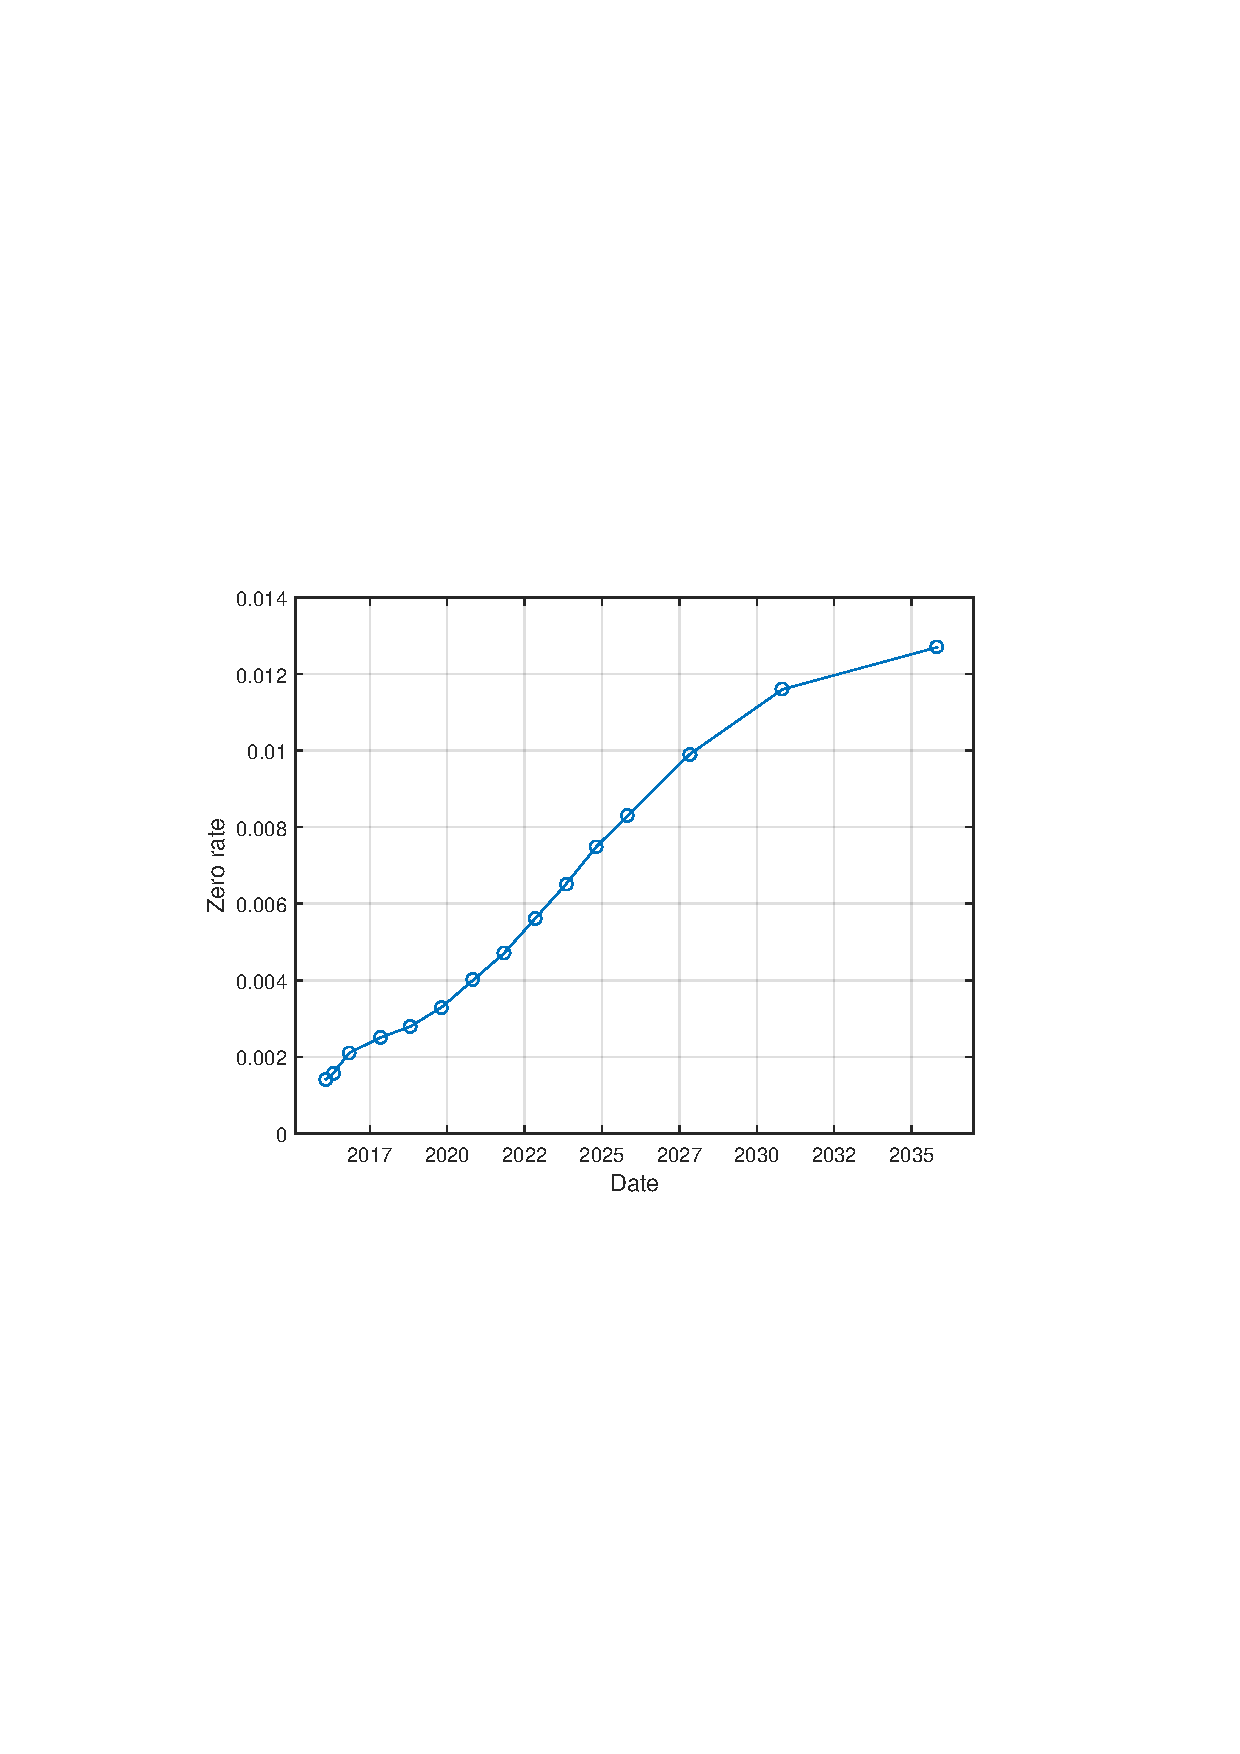
\includegraphics[width=6cm, clip, trim= 110 270 110 270]{IMG/YieldCurve.pdf}
  \caption{Yield Curve}  \label{YieldCurve}
\end{figure}

\subsection{Interest rate simulation}
The interest rate simulation is based on historical data of the three month PRIBOR rate, from 2. 1. 2014 to 24. 11. 2015.  
The development of three month PRIBOR rate can be observed in the figure \ref{PRIBOR}.

\begin{figure}[!htbp]
  \centering 
	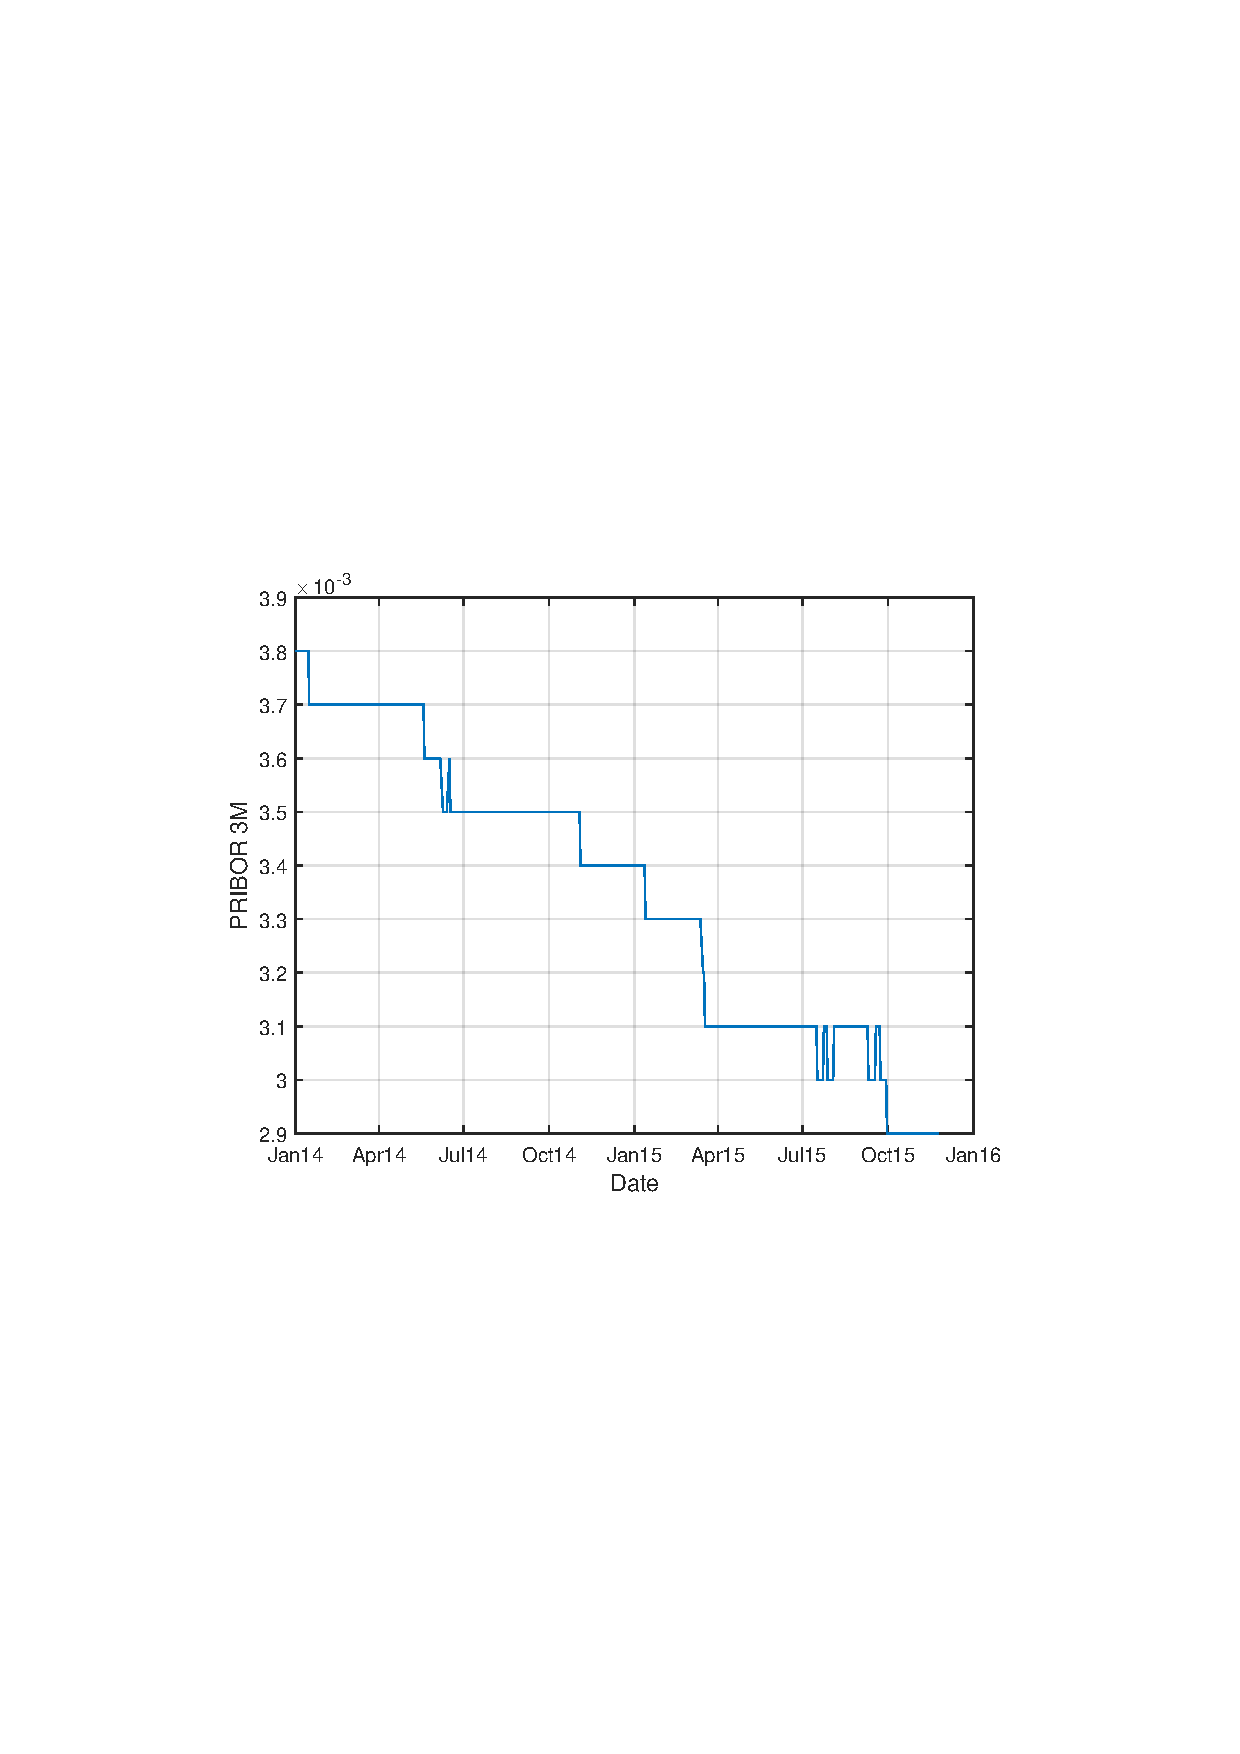
\includegraphics[width=6cm, clip, trim= 110 270 110 270]{IMG/PRIBOR.pdf}
  \caption{The three month PRIBOR rate}  \label{PRIBOR}
\end{figure}

The well known interest rate evolution model, Hull-White one-factor model, will be used for modeling of the interest rate term structure. 
%The Hull-White model is a one-factor model of the short rate $r(t)$, first published in \cite{hull1990pricing} and generalized later \cite{hull2001general}.
The model was first published by John Hull and Alan White in \cite{hull1990pricing} and generalized later in \cite{hull2001general}.
%The need for an exact fit to the currently-observed yield curve, led Hull and White to the introduction of a time-varying parameter in the Vasicek model. 
The requirement for more accurate fit to the currently-observed yield curve, led Hull and White to the introduction of a time variable parameter in the Vasicek model. 
%The model assumes that short rates have a normal distribution, and that the short rates are subject to mean reversion.
The model assumes that short rates have a normal distribution, and also that the short rates exhibit the mean reversion character. 
%Volatility is likely to be low when short rates are near zero, which is reflected in a larger mean reversion in the model. 
The Hull-White model extends the Vasicek and Cox-Ingersoll-Ross (CIR) models.

We can define this model by equation
\begin{equation}
\dr(t)=[\theta(t)-\alpha r]\dt+\sigma\dW,
\label{H-Wmodel}
\end{equation}
where
\begin{description}
\item [$\dr$] The change in the interest rate after a small change in time, $\dt$.
\item [$\alpha$   ] Constant reversion speed.%Mean reversion rate.
\item [$\sigma$   ] Volatility of the interest rate.
\item [$\dW$] A Wiener process.
\item [$\theta(t)$] Drift function defined as
\begin{equation}
\theta(t)=\frac{\partial  F(0,t)}{\partial t}+\alpha F(0,t)+\frac{\sigma^2}{2 \alpha}(1-\e^{-2\alpha t}), %F'_{t}(0,t)+...
\end{equation}
where
\item[$F(0,t)$] Instantaneous forward rate at time $t$.
%\item[$F'_{t}(0,t)$] Partial derivative of $F$ with respect to time $t$.
\end{description}
Instantaneous forward rate $F(0,t)$ is defined as
\begin{equation}
F(0,t)= \frac{\partial\ln  P(0,t)}{\partial t}
\end{equation}
where $ P(t,T)$ is price of a zero coupon bond at time $t$ with maturity at time $T$.

The constants $\alpha$ and $\sigma$ are extracted from the historical three month PRIBOR rates.
We use equation \eqref{H-Wmodel} to simulated the short interest rates.  
We can expand the entire interest rate curve from the short rate using
\begin{eqnarray}
%R(t,T)&=&-\frac{1}{T-t}\ln A(t,T)+\frac{1}{T-t}B(t,T)r(t)\\
P(t,T)&=&A(t,T)\e^{-B(t,T)r(t)}\\
\ln A(t,T)&=&\ln \frac{P(0,T)}{P(0,t)}+B(t,T)F(0,t)-\frac{1}{4\alpha^3}\sigma^2(\e^{-\alpha T}-\e^{-\alpha t})^2(\e^{2\alpha t}-1)  \nonumber\\
B(t,T)&=&\frac{1-\e^{-\alpha(T-t)}}{\alpha}.\nonumber
\end{eqnarray}
The large number of simulations was made. 
The example of yield surfaces obtained in one interest rate simulation is possible to observe in the Figure \ref{YieldCurveEvolution}.
\begin{figure}[!htbp]
  \centering 
	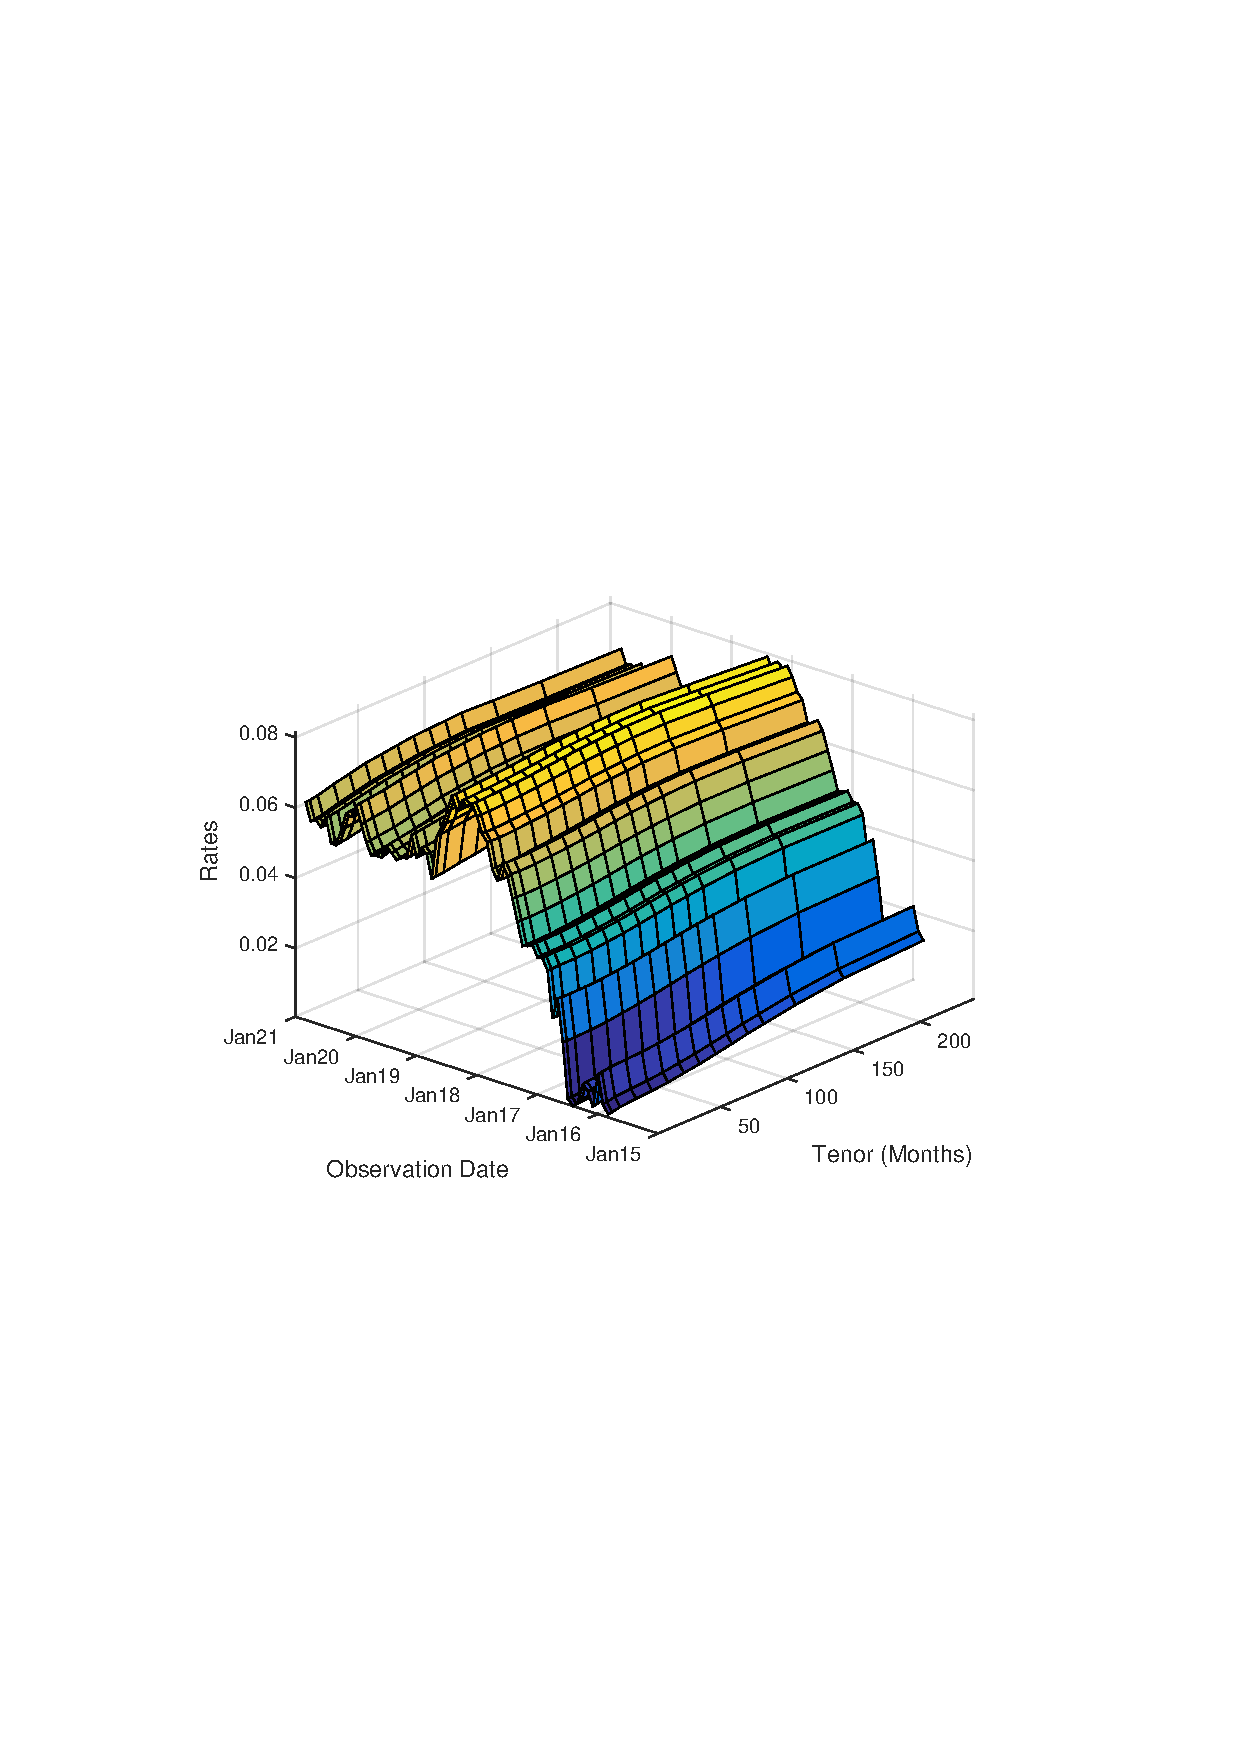
\includegraphics[width=6cm, clip, trim= 110 270 110 270]{IMG/YieldCurveEvolution.pdf}
  \caption{ One Possible Scenario of Yield Curve Evolution}  \label{YieldCurveEvolution}
\end{figure}
For each scenarios the swaps are priced at each future simulation date. 

The main advantage of the Hull-White model is that it can be fitted exactly to the initial term structure of interest rates.

\subsection{Probability of default}
We assume that the wait time for default of a counterparty is a random variable $X$ with exponential distribution. Then the cumulative distribution function of this variable can be define as
\begin{equation}
F(x)= P(X\leq x)= \left\{ \begin{array}{r@{\quad}c}
    1-\e^{-\lambda x}, & x \geq 0 \\
    0, & x \leq 0 \\ \end{array} \right.
    \label{exponentialdistr}
\end{equation}
where $\lambda>0$ is the parameter of the distribution. Probability of default of the counterparty during one year we denote $PD$. Then 
\begin{equation}
PD=P(X\leq 1)=1-\e^{-\lambda}.
\label{PD}
\end{equation}
If we use value of PD from \textcolor{red}{odkud bereme PD, Leni?}  $\lambda$ could be estimate from \eqref{PD} 
\begin{eqnarray}
PD&=&1-\e^{-\lambda} \nonumber \\
\lambda&=&-\ln(1-PD).
\end{eqnarray}
Then we can construct probability curve for each counterparty. It is possible to observed them in the Figure \ref{DefaultProbability}.

\begin{figure}[!htbp]
  \centering 
	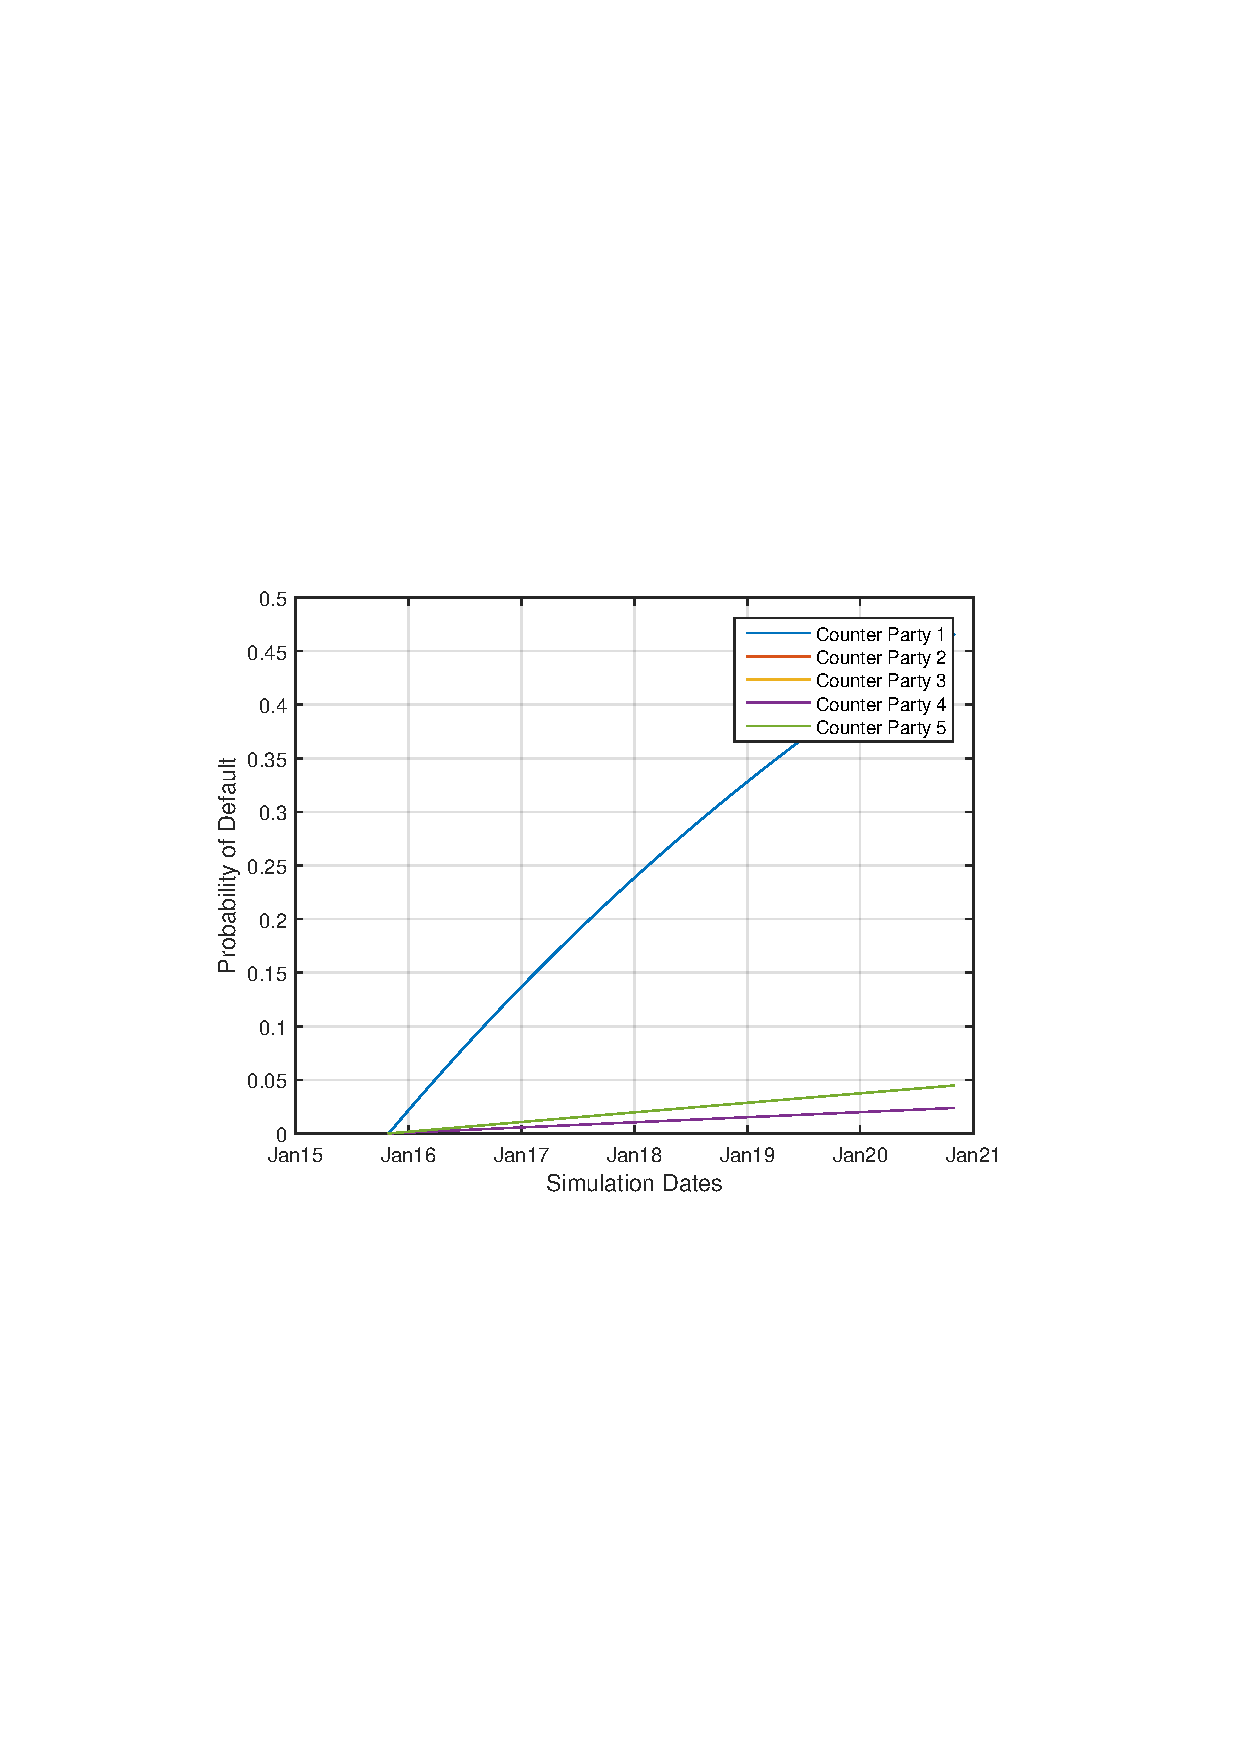
\includegraphics[width=6cm, clip, trim= 110 270 110 270]{IMG/DefaultProbability.pdf}
  \caption{Default Probability Curves}  \label{DefaultProbability}
\end{figure}


\subsection{Computation of CVA} 
Let consider the exposure is independent of default. Then total exposure of all contracts can be computed on the bases of equation \eqref{totalExposure}. The bank has estimated recovery rate $R=40\%$. \textcolor{red}{Leni, jaká je vaše recovery rate?}. Now we have everything for the CVA calculation according to the equation \eqref{CVA}. The resulting values of CVA for each counterparty can be observed in the Table \ref{resultingCVA}.

\begin{table}
\scalebox{1}{\begin{tabular}{|c |r|}
\hline
\textbf{Counterparty} &\textbf{CVA (in CZK)}\\ 
\hline
$\boldsymbol{1}$ &1 056 075.83  \\ 
$\boldsymbol{2}$&265 290.14  \\
$\boldsymbol{3}$&369.19 \\
$\boldsymbol{4}$& 1 045.54\\
$\boldsymbol{5}$&103 319.55 \\
\hline
\end{tabular}}
\vspace{0,5cm}
\caption{Resulting CVA}
\label{resultingCVA}
\end{table}



\begin{comment}
\begin{figure}[!htbp]
  \centering 
	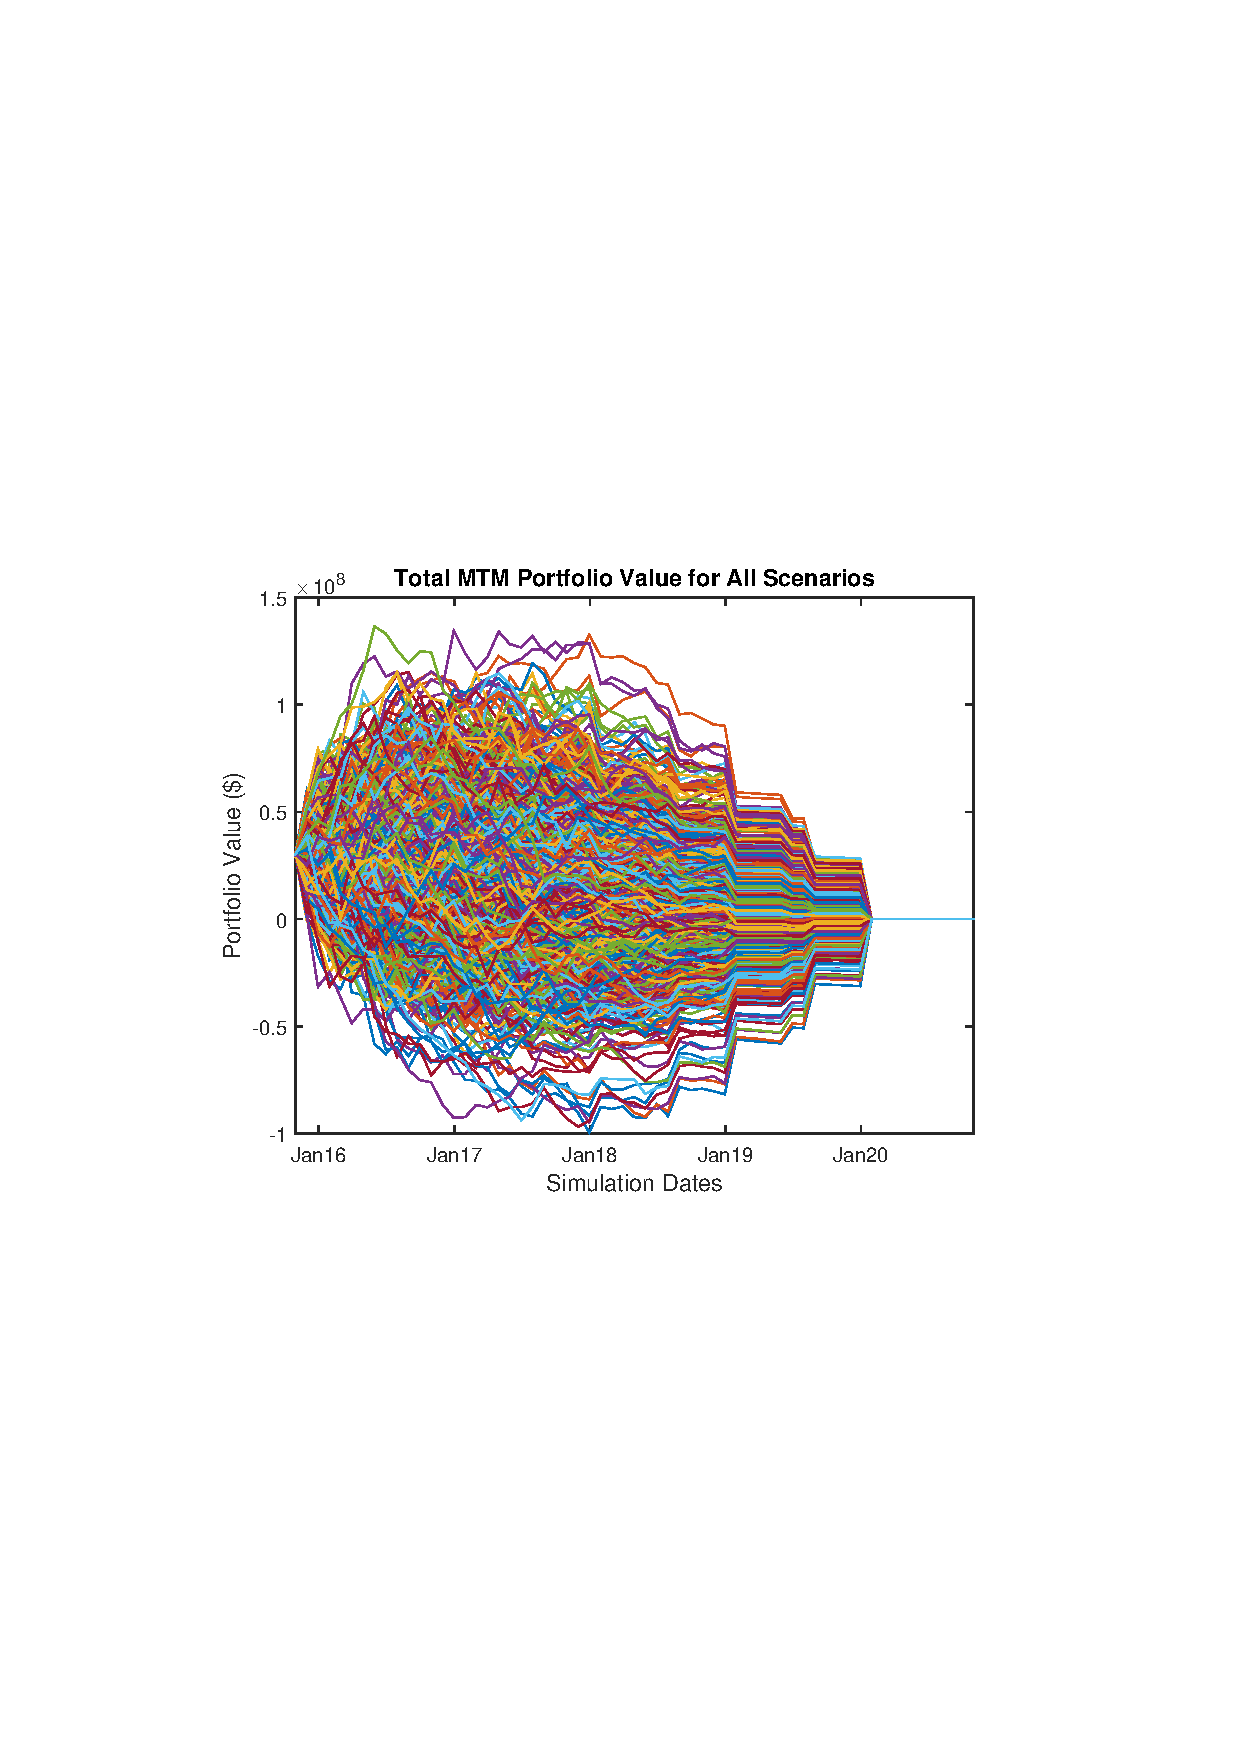
\includegraphics[width=6cm, clip, trim= 110 270 110 270]{IMG/TotalPortfoioValue.pdf}
  \caption{Total Portfoio Value}  \label{TotalPortfoioValue}
\end{figure}

\begin{figure}[!htbp]
  \centering 
	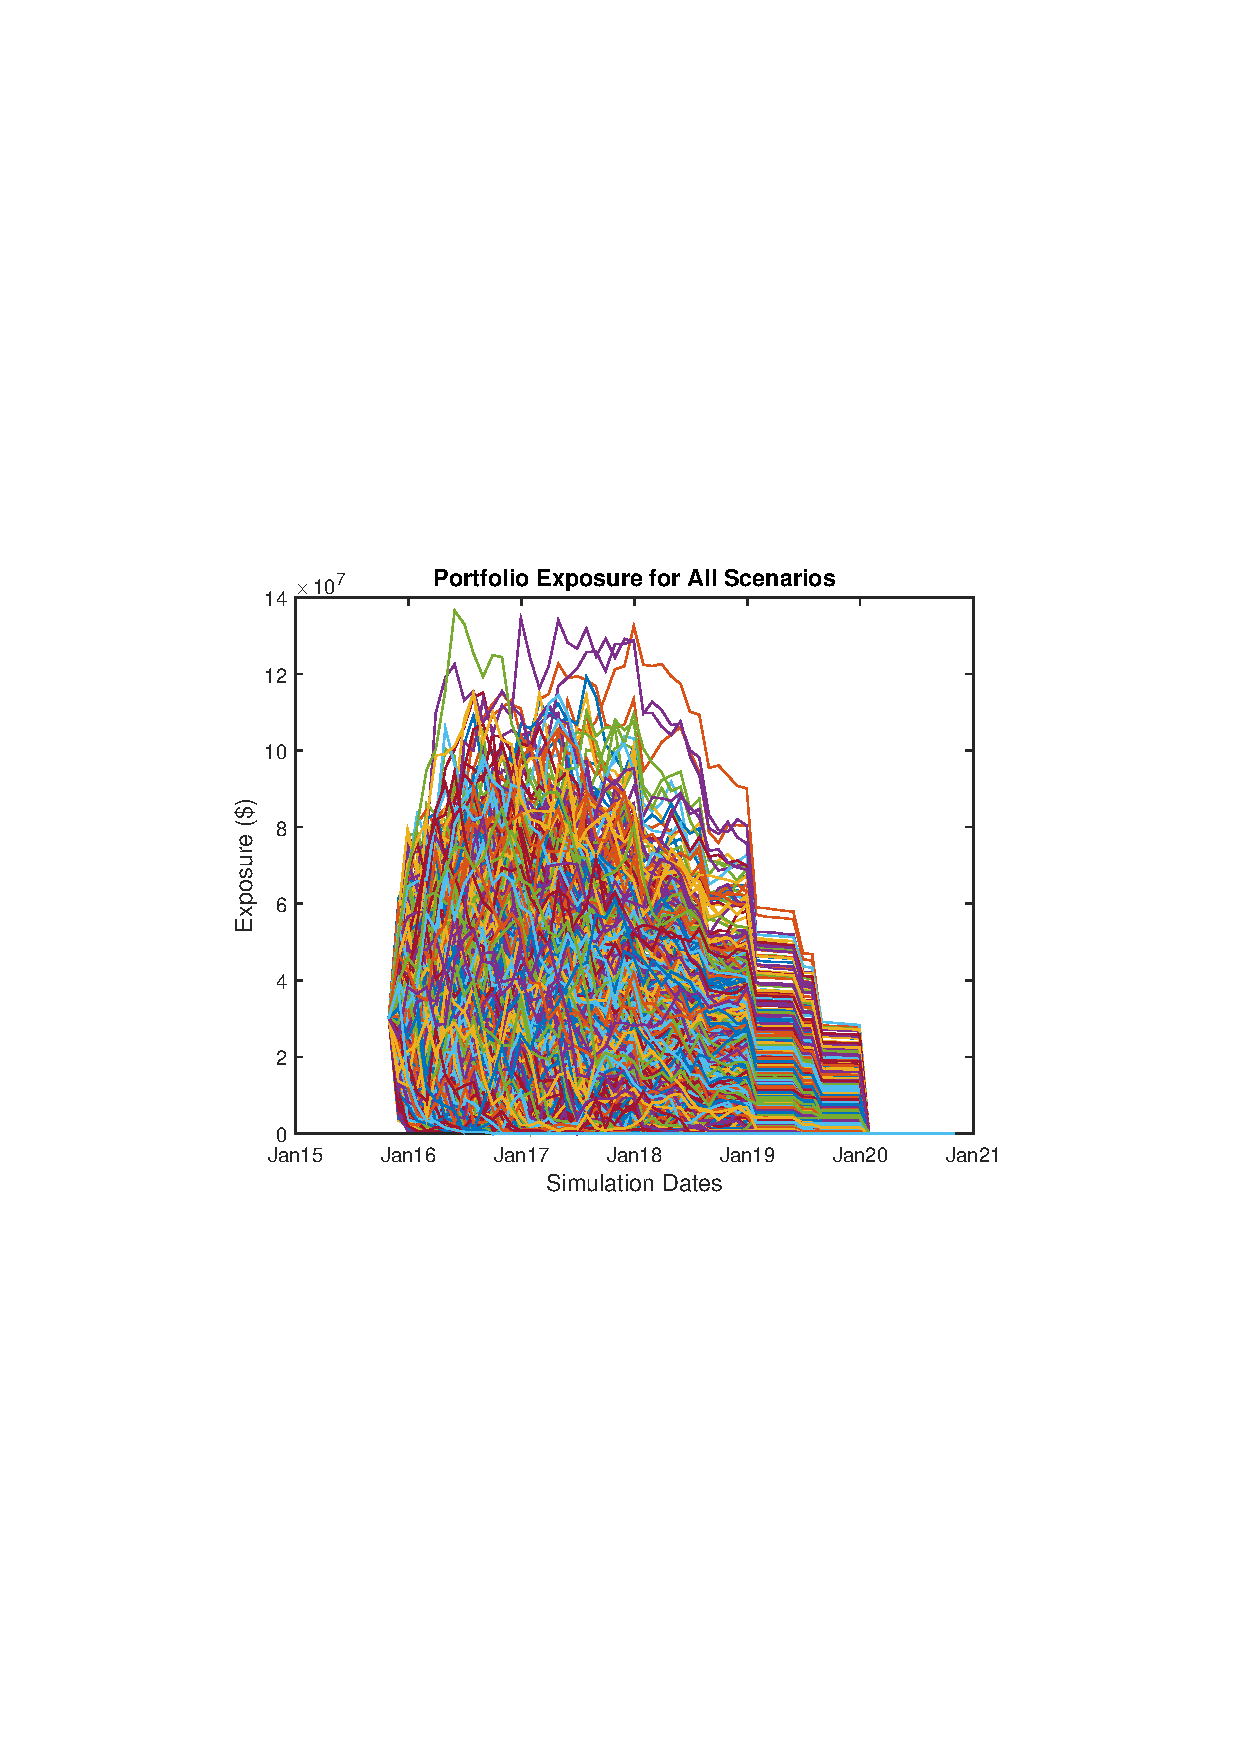
\includegraphics[width=6cm, clip, trim= 110 270 110 270]{IMG/PorfolioExposure.pdf}
  \caption{Porfolio Exposure}  \label{PorfolioExposure}
\end{figure}

\begin{figure}[!htbp]
  \centering 
	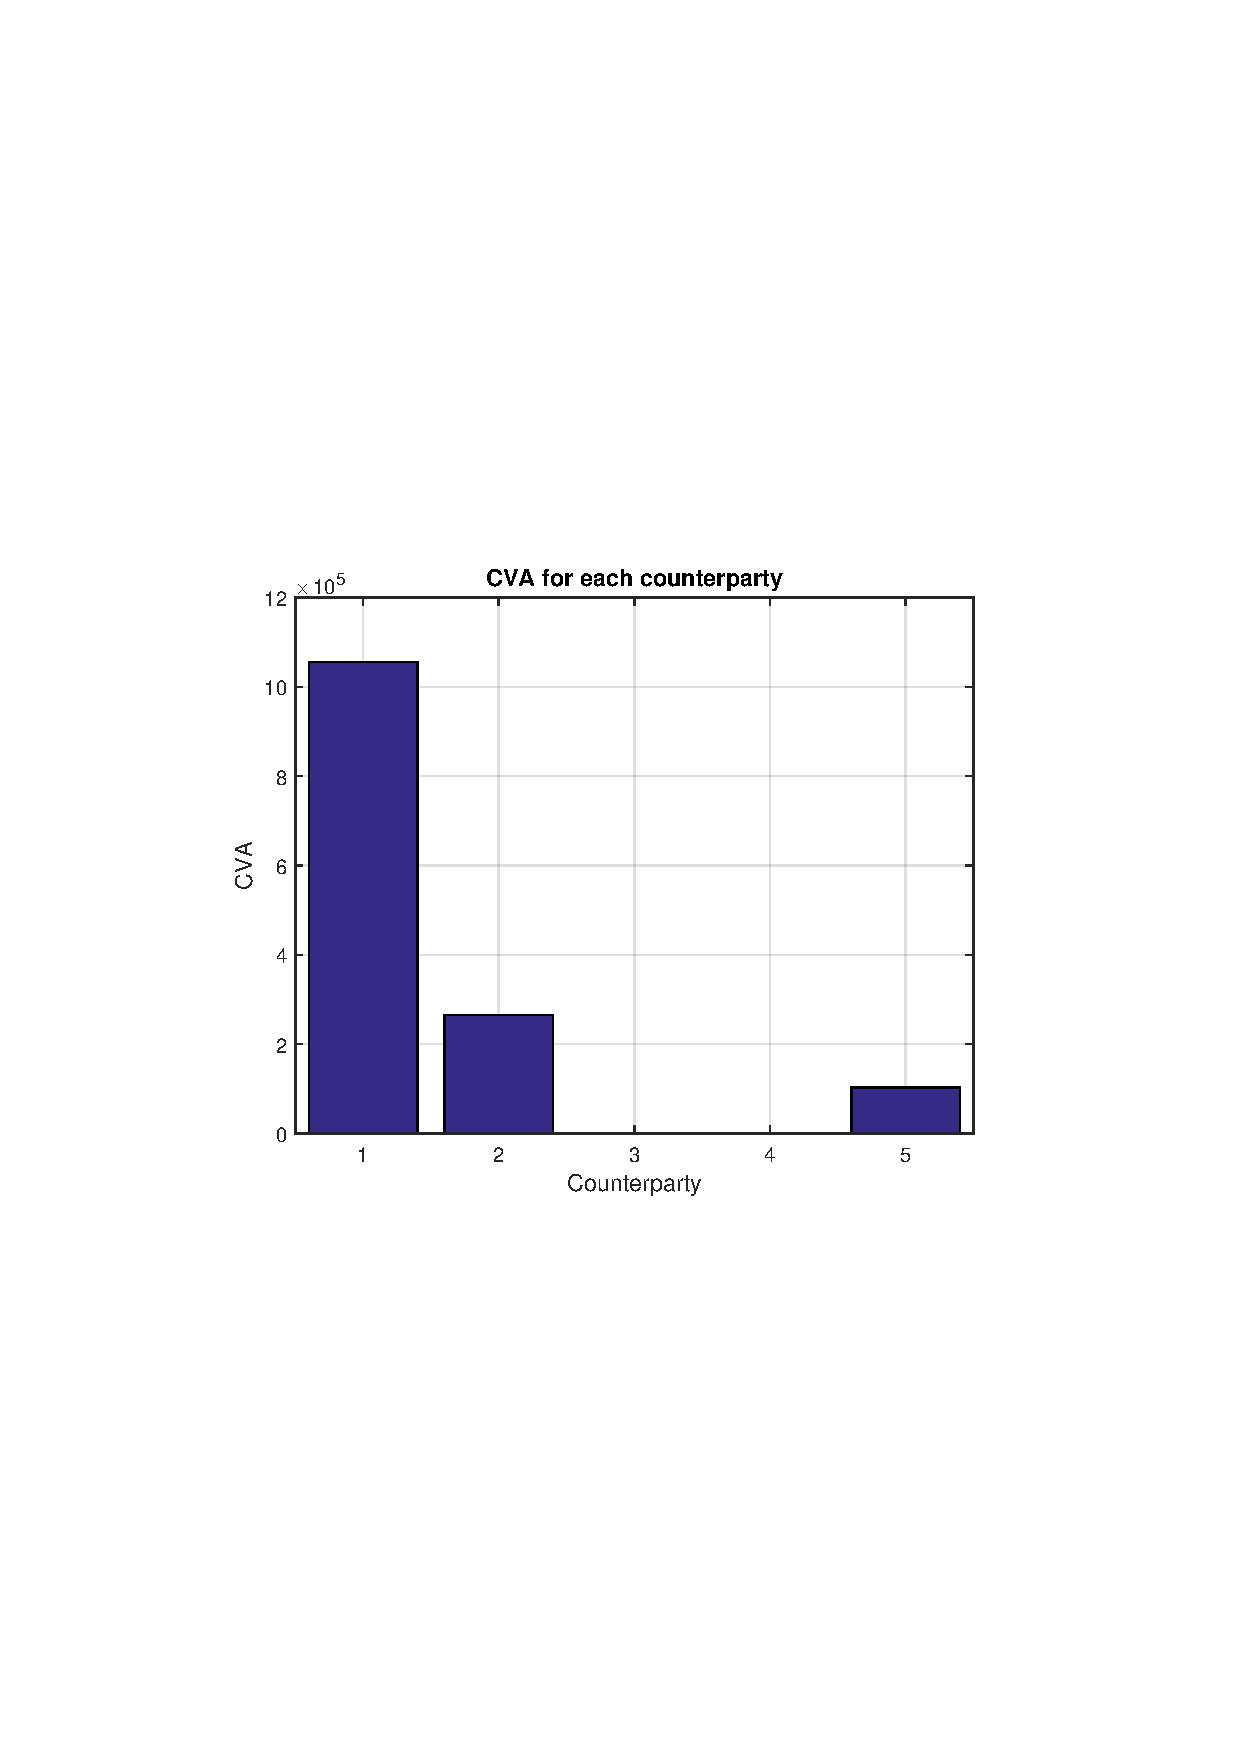
\includegraphics[width=6cm, clip, trim= 110 270 110 270]{IMG/CVAforEachCounterparty.pdf}
  \caption{CVA for each counterparty}  \label{CVAforEachCounterparty}
\end{figure}
\end{comment}




%\section{Methods of Comparing Different Models}
%\subsection{Analysis of Deviance}
%\subsection{Information Criteria}
%\section{Applying Generalized Linear Models in Actuarial Science}

%\begin{comment}
\begin{thebibliography}{99}
\bibitem{arora2012}
N.~Arora, P.~Gandhi, and F.~A. Longstaff.
\newblock Counterparty credit risk and the credit default swap market.
\newblock {\em Journal of Financial Economics}, 103(2):280--293, 2012.

\bibitem{bouchaud2003theory}
J.-P. Bouchaud and M.~Potters.
\newblock {\em Theory of financial risk and derivative pricing: from
  statistical physics to risk management}.
\newblock Cambridge university press, 2003.

\bibitem{brigo2014}
D.~Brigo, A.~Capponi, and A.~Pallavicini.
\newblock Arbitrage-free bilateral counterparty risk valuation under
  collateralization and application to credit default swaps.
\newblock {\em Mathematical Finance}, 24(1):125--146, 2014.

\bibitem{canabarro2003measuring}
E.~Canabarro and D.~Duffie.
\newblock Measuring and marking counterparty risk.
\newblock {\em Asset/Liability Management for Financial Institutions,
  Institutional Investor Books}, 2003.

\bibitem{duffie2003intertemporal}
D.~Duffie.
\newblock {\em Intertemporal asset pricing theory}, volume~1.
\newblock Elsevier, 2003.

\bibitem{etheridge2002course}
A.~Etheridge.
\newblock {\em A course in financial calculus}.
\newblock Cambridge University Press, 2002.

\bibitem{gregory2010}
J.~Gregory.
\newblock {\em Counterparty credit risk: the new challenge for global financial
  markets}, volume 470.
\newblock John Wiley \& Sons, 2010.

\bibitem{hull}
J.~Hull.
\newblock {\em Options, futures, and other derivatives (8. ed., global ed.)}.
\newblock Boston [u.a.] : Pearson, 2012.

\bibitem{hull1990pricing}
J.~Hull and A.~White.
\newblock Pricing interest-rate-derivative securities.
\newblock {\em Review of financial studies}, 3(4):573--592, 1990.

\bibitem{hull2001general}
J.~Hull and A.~White.
\newblock The general hull-white model and supercalibration.
\newblock {\em Financial Analysts Journal}, 57(6):34--43, 2001.

\bibitem{hull2012cva}
J.~Hull and A.~White.
\newblock Cva and wrong-way risk.
\newblock {\em Financial Analysts Journal}, 68(5):58--69, 2012.

\bibitem{jilek2000}
J.~J{\'i}lek.
\newblock Finan{\v{c}}n{\'\i} rizika. 1. vyd. praha: Grada, 2000. 635 s.
\newblock Technical report, ISBN 80-7169-579-3, 2000.

\bibitem{pykhtin2010}
M.~Pykhtin and D.~Rosen.
\newblock Pricing counterparty risk at the trade level and cva allocations.
\newblock 2010.

\end{thebibliography}
%\end{comment}

%\nocite{bouchaud2003theory} 
%\nocite{duffie2003intertemporal} 
%\nocite{etheridge2002course} 
%\nocite{hull} 
%\nocite{pykhtin2010} 
%\nocite{gregory2010} 
%\nocite{brigo2014} 
%\nocite{hull2012cva} 
%\nocite{arora2012} 
%\nocite{jilek2000} 
%\nocite{canabarro2003measuring} 


%\nocite{}  %umisti do literatury i necitovanou polozku a \nocite{*} umisti do literatury vsechny polozky z bibtex databaze 

%\bibliographystyle{plain}
%\bibliographystyle{abbrv}
%\bibliography{bibliography}

\end{document}